%% \VignetteIndexEntry{Bioconductor LaTeX Style}

\documentclass{article}

\RequirePackage{/home/muhammad/R/x86_64-pc-linux-gnu-library/3.0/BiocStyle/sty/Bioconductor}\newcommand{\exitem}[3]{\item \texttt{\textbackslash#1\{#2\}} #3 \csname#1\endcsname{#2}.}

\title{A probabilistic dynamical model for quantitative inference of the regulatory mechanism of transcription}
\author{Guido Sanguinetti, Magnus Rattray and Neil D. Lawrence}
%%\author{Muhammad A. Rahman}

\usepackage{Sweave}
\begin{document}
\Sconcordance{concordance:chipDyno.tex:chipDyno.Rnw:%
1 3 1 1 4 6 1 1 0 39 1 1 3 2 0 1 1 5 0 1 5 4 0 3 1 13 0 1 2 2 1 1 2 1 0 5 1 13 0 %
1 2 2 1 1 3 2 0 1 6 4 0 6 1 3 0 1 2 2 1 1 2 1 0 1 6 4 0 6 1 6 0 1 2 2 1 1 2 1 0 %
1 4 3 0 3 1 3 0 1 2 1 1 1 3 2 0 1 6 4 0 1 2 2 1 3 0 1 2 2 1 1 2 1 0 1 5 3 0 4 1 %
3 0 1 2 2 1 1 2 1 0 1 5 3 0 2 1 3 0 1 2 1 1 1 2 1 0 1 1 1 6 4 0 1 2 3 1 1 4 2 0 %
1 1 1 5 4 0 1 7 5 0 2 1 4 0 1 3 107 1 1 2 1 0 1 1 3 0 1 2 10 1 1 2 10 0 1 2 8 1}


\maketitle

\begin{abstract}
Quantitative estimation of the regulatory relationship between transcription factors and genes is a fundamental stepping stone when trying to develop models of cellular processes. This task, however, is difficult for a number of reasons: transcription factors` expression levels are often low and noisy, and many transcription factors are post-transcriptionally regulated. It is therefore useful to infer the activity of the transcription factors from the expression levels of their target genes.
\end{abstract}

\tableofcontents

\section{Installing the \Biocpkg{chipDyno} package}
The recommended way to install the \Bioconductor{} package \Biocpkg{chipDyno} is to use the \Rfunction{biocLite} function available in the \Bioconductor{} website. This way of installation should ensure that all the dependencies are met.

\begin{verbatim}
    > source ("www.//bioconductor.org/chipDyno.R")
    > biocLite("chipDyno")
\end{verbatim}

%%To determine the gene specific transcription factor activity of C. Elegans we have followd Sanguinetti's probabilistic dynamic model ~\cite{sanguinetti:01} for quantative inference.

\section{Loading the package and getting help}
The first step in any \Biocpkg{chipDyno} analysis is to load the package. This package can be loaded when the \R{} console is ready. At the \R{} console type the following command:

\begin{verbatim}
    > library("chipDyno")
\end{verbatim}

Command \Rfunction{help} can be used to get help on any function. For example, to get help on the \Rfunction{chipDynoLikeStatGrad} type the following (both of them have the similar output):

\begin{verbatim}
    > help(chipDynoLikeStatGrad)
    > ?chipDynoLikeStatGrad
\end{verbatim}


\section{Input data and preparations}
If the data is in Affymetrix CEL files then it may required to do some preprocessing. This CEL files can be extracted using the bioconductor package \Biocpkg{puma} ~\cite{puma}. \Biocpkg{puma} usually stores the point expression in \file{*\_exprs.csv} file and defferent levels of uncertainties in \file{*\_se.csv} files as Comma-separated values.

Load the point expression levels data and it corresponding uncertainty. Here the data was stored in a simple text file %\file{YeastMetabolism_exprs.txt} and \file{YeastMetabolism_se.txt} respectively.

\begin{Schunk}
\begin{Sinput}
> rm(list=ls())
> source("/home/muhammad/Dropbox/Git/mlprojects/chipDyno/R/chipDynoLoadModules.R")
> file_data <- 
+   "/home/muhammad/Dropbox/Git/mlprojects/chipDyno/R/data/MetabolData/YeastMetabolism_exprs.txt";
> file_vars <- 
+   "/home/muhammad/Dropbox/Git/mlprojects/chipDyno/R/data/MetabolData/YeastMetabolism_se.txt";
> data = as.matrix(read.table(file_data))
> data[1:5,1:8]
\end{Sinput}
\begin{Soutput}
            V1        V2        V3        V4        V5         V6         V7         V8
[1,]  3.032196  3.915297  3.513140  2.887694  2.624707  2.4336185  0.5146789  3.0277957
[2,]  7.619968  7.009363  6.327303  6.420305  6.474659  6.4259952  5.9848784  6.6202407
[3,]  9.367415  9.337176  9.346070  9.528845  9.870827  9.9068906  9.2679571  9.7358944
[4,] 11.116018 10.157765 10.559681 10.625835 10.832905 11.1418061 10.7627800 11.1802351
[5,] -1.746557 -1.909657  1.074617 -2.313146 -1.508921 -0.9244119 -1.7330923 -0.8551462
\end{Soutput}
\begin{Sinput}
> vars=as.matrix(read.table(file_vars))
> vars[1:5,1:8]
\end{Sinput}
\begin{Soutput}
            V1        V2        V3        V4        V5         V6        V7         V8
[1,] 0.5988238 0.3692819 0.4940527 0.6459059 0.8544423 0.82382426 1.4128785 0.62460252
[2,] 0.1291985 0.1683352 0.2438547 0.2245224 0.2532125 0.23656530 0.2989101 0.21290733
[3,] 0.0000000 0.0000000 0.0000000 0.0000000 0.0000000 0.00000000 0.0000000 0.00000000
[4,] 0.1019400 0.1426169 0.1248059 0.1224968 0.1122887 0.09996799 0.1154624 0.09959699
[5,] 1.8253530 1.8705859 0.9995836 1.9992325 1.8095992 1.60575819 1.8439322 1.57351633
\end{Soutput}
\end{Schunk}

These differentially expressed data and its uncertainty doesn't contain any genes name or problem ID number. The gene Names and its corresponding  problem IDs can be extracted from other two source (?) dictionary.txt and probeIDTu.txt.

\begin{Schunk}
\begin{Sinput}
> file_dictionary <- 
+   "/home/muhammad/Dropbox/Git/mlprojects/chipDyno/R/data/MetabolData/dictionary.txt";
> dictionary <- read.table(file_dictionary, header = FALSE, sep = "\t", 
+     		quote = "", dec = ".", col.names=c("IDs_temp", "ORF", 
+ 				"ORF_temp","geneCN_temp"), na.strings = "NA", 
+ 				colClasses = NA, nrows = -1, skip = 0, check.names = TRUE, 
+ 				fill = TRUE, strip.white = FALSE, blank.lines.skip = FALSE, 
+ 				comment.char = "#", allowEscapes = FALSE, flush = FALSE)
> IDs= matrix(dictionary$IDs_temp,,1)
> ORF= matrix(dictionary$ORF,,1) 
> file_probeIDTu <- 
+   "/home/muhammad/Dropbox/Git/mlprojects/chipDyno/R/data/MetabolData/probeIDTu.txt";
> probeIDTu <- read.table(file_probeIDTu, sep=" ", fill= TRUE, col.names=c("IDSn"))
> IDSnew <- matrix(probeIDTu$IDSn,,1)
\end{Sinput}
\end{Schunk}


%In our experimental data set there was 3 replication of the same experiment with 5 experimental time points with different environmental conditions. So there was (3x5=) 15 time points. We will to reorganize this datapoint maintaining the time series for different experiment. For our this example we will consider the data obtained from the second experiment.

%Load the the standard errors. The ~\cite{puma} package creates many files with different percentile of posterior destribution we can choose anyone based on our requirement. Here as well we are considering the second experiment

The connectivity contains the evidence of connectivity between a gene and a transcription factor. \Rcode{Connectivity2.txt} file depicts the relation between 6229 genes and 204 transcription factors.  Load the connectivity file.
\begin{Schunk}
\begin{Sinput}
> file_dataChip <- 
+   "/home/muhammad/Dropbox/Git/mlprojects/chipDyno/R/data/Connectivity2.txt";
> dataChip=as.matrix(read.table(file_dataChip))
\end{Sinput}
\end{Schunk}

From the annotation file we can find the gene names present in the connectivity information. Load the annotation file. % For annotation we used ~\cite{celegans:db}.
\begin{Schunk}
\begin{Sinput}
> file_annotation <- 
+   "/home/muhammad/Dropbox/Git/mlprojects/chipDyno/R/data/annotations2.txt"
> probe_anno <- read.table(file_annotation, header = FALSE, sep = "\t", quote = "", 
+                          dec = ".", col.names=c("prob", "anno"), na.strings = "NA", 
+                          colClasses = NA, nrows = -1, skip = 0, check.names = TRUE, 
+                          fill = TRUE, strip.white = FALSE, blank.lines.skip = FALSE, 
+                          comment.char = "#", allowEscapes = FALSE, flush = FALSE)
> probeName2=matrix(probe_anno$prob,,1) 
> annota=matrix(probe_anno$anno,,1)
\end{Sinput}
\end{Schunk}

The list of transcription factors present in the connectivity information can be found from the file %Trans_Names2.txt . Load the file.   

\begin{Schunk}
\begin{Sinput}
> file_transNames <- 
+   "/home/muhammad/Dropbox/Git/mlprojects/chipDyno/R/data/Trans_Names2.txt"
> TransNames_tab <- read.table(file_transNames, header = FALSE, sep = "\t", quote = "", 
+                              dec = ".", col.names=c("TN"), na.strings = "NA", 
+                              colClasses = NA, nrows = -1, skip = 0, check.names = TRUE, 
+                              fill = TRUE, strip.white = FALSE, blank.lines.skip = FALSE,
+                              comment.char = "#", allowEscapes = FALSE, flush = FALSE)
> TransNames = matrix(TransNames_tab$TN,,1)
\end{Sinput}
\end{Schunk}

In our experimental data set there are some genes for which the measurement of uncertainty is zero(i.e. vars[3,]). We would like to exclude those data.
\begin{Schunk}
\begin{Sinput}
> zeroValueRow = which(rowSums(vars)==0)
> data = data[-zeroValueRow, ]
> vars = vars[-zeroValueRow, ]
> probeName = ORF # Rename ORF
> probeName = matrix(probeName[-zeroValueRow, ],,1)
\end{Sinput}
\end{Schunk}

All the genes represent the connectivity information with the transcription factors might not present in the differentially expressed data set. We will like to exclude those genes. The following segment of code will exclude those genes. We will also exclude the redundant genes, their point expression data and uncertainty levels.
\begin{Schunk}
\begin{Sinput}
> noOfprobe=nrow(probeName)
> redundancy=matrix(mat.or.vec(noOfprobe,1),,1)
> redundancy[,]=1
> index=matrix(mat.or.vec(nrow(dataChip),1),,1)
> for (i in 1: nrow(probeName2)){
+ 	vec <- probeName==probeName2[i,1]
+ 	index[i]=colSums(vec)
+ 	if(index[i]>1){
+ 		pippo=(which(vec))
+ 		redundancy[pippo[2:length(pippo)]]=0
+ 		}
+ 	}
> dataChip=dataChip[which(index!=0),]
> annota=annota[which(index!=0),]
> probeName2=probeName2[which(index!=0),]
> probeName2=matrix(probeName2,,1)
> probeName=probeName[which(redundancy!=0),]
> probeName=matrix(probeName,,1)
> data=data[which(redundancy!=0),]
> vars=vars[which(redundancy!=0),]
\end{Sinput}
\end{Schunk}

Again all the genes have the differentially expressed data may not have the connectivity information with the transcription factors. We will exclude those genes as well. We will also organize the genes connectivity information based on the differentially expressed genes index. So that in both data set (points expressions with uncertainty and connectivity information) have the common genes and aligned with the same index.

\begin{Schunk}
\begin{Sinput}
> preX=NULL
> annotation=NULL
> index=mat.or.vec(nrow(data),1)
> for (i in 1: nrow(data)){
+ 	index[i]=sum(probeName[i]==probeName2)
+ 	if (index[i]==1)		
+ 		preX=rbind(preX,dataChip[which(probeName[i]==probeName2),])
+ 		annotation=rbind(annotation,annota[which(probeName[i]==probeName2)])
+ }
> data= data[which(index==1),]
> vars= vars[which(index==1),]
> probeName= probeName[which(index==1),]
> probeName=matrix(probeName,,1)
\end{Sinput}
\end{Schunk}

The connectivity matrix between genes and the transcription factors is a binary matrix. If there is an evidence that a gene is transcribed by a transcription factor or, a transcription factor is transcribing some other genes then the relation will be 1, the value will be 0 otherwise. We binarized the matrix by giving a value based on the suggestion of ~\cite{lee:01} when the associated p-value is less than 0.0001.
\begin{Schunk}
\begin{Sinput}
> X= mat.or.vec(nrow(preX),ncol(preX))
> I <- c(which(preX<1e-3))
> X[I] =1
\end{Sinput}
\end{Schunk}

In the experimental dataset there might have some genes which are not transcribing by any of the given transcription factors, again there might have some transcription factors which are not transcribing any of the present genes. We will exclude those genes and transcription factors.
\begin{Schunk}
\begin{Sinput}
> fakeX = rowSums(X)
> X=X[which(fakeX!=0),]
> annotation=annotation[which(fakeX!=0),]
> annotation = matrix(annotation,,1)
> effectX=colSums(X)
> TransNames=TransNames[which(effectX!=0),]
> TransNames=matrix(TransNames,,1)
> X=X[,which(effectX!=0)]; X[201:207,16:30]
\end{Sinput}
\begin{Soutput}
     [,1] [,2] [,3] [,4] [,5] [,6] [,7] [,8] [,9] [,10] [,11] [,12] [,13] [,14] [,15]
[1,]    0    0    0    0    0    1    0    0    0     0     0     0     0     0     0
[2,]    0    1    0    0    0    0    0    0    0     0     0     0     0     0     0
[3,]    0    0    0    0    0    1    0    0    0     0     0     0     1     0     0
[4,]    0    0    0    0    0    0    0    0    0     0     0     0     0     0     0
[5,]    0    0    0    0    0    1    0    0    0     0     0     0     1     0     0
[6,]    0    0    0    0    0    0    0    0    0     0     0     0     0     0     0
[7,]    0    0    0    0    0    0    0    0    0     0     0     0     0     0     0
\end{Soutput}
\begin{Sinput}
> data= data[which(fakeX!=0),]; data[1:5,1:7]
\end{Sinput}
\begin{Soutput}
             V1          V2        V3        V4         V5          V6         V7
[1,]  7.6199683  7.00936333  6.327303  6.420305  6.4746593  6.42599518  5.9848784
[2,] 11.1160178 10.15776528 10.559681 10.625835 10.8329051 11.14180612 10.7627800
[3,]  5.6794099  5.94811239  5.656218  6.013510  6.6347741  6.82920197  6.4394373
[4,] -0.8461938 -0.09323972  1.174838  2.204736  0.7630712  0.05440951  0.9871222
[5,] 11.2509533 11.10515487 10.940308 10.467595 10.3794020  9.96586556  9.8538724
\end{Soutput}
\begin{Sinput}
> vars= vars[which(fakeX!=0),]; vars[1:5,1:7]
\end{Sinput}
\begin{Soutput}
             V1         V2         V3         V4         V5         V6        V7
[1,] 0.12919850 0.16833525 0.24385468 0.22452239 0.25321253 0.23656530 0.2989101
[2,] 0.10194004 0.14261692 0.12480590 0.12249678 0.11228873 0.09996799 0.1154624
[3,] 0.35203433 0.30378077 0.36894665 0.29941130 0.24717867 0.20727438 0.2476667
[4,] 2.14604703 1.89233701 1.47218035 1.15147407 1.67454729 1.86261881 1.5501621
[5,] 0.06955393 0.07214869 0.07750579 0.09116104 0.09549444 0.10993607 0.1157719
\end{Soutput}
\end{Schunk}

Define some variables-
\begin{Schunk}
\begin{Sinput}
> nGenes= nrow(data) # Number of genes will be present in our experiment
> npts= ncol(data) # Number of time points
> nTrans = ncol(X) # Number of TF will be present in our experiment
> muIn = array(0, dim <-c(nTrans,1)); 
> annotations = annotation # Both of the variavle contain the same data
> transNames = TransNames # Both of the variavle contain the same data
\end{Sinput}
\end{Schunk}

\section{Reduce Variables}
The connectivity matrix is a sparse matrix. Using \Rfunction{chipReduceVariables} we can find the same length integer vectors having the row indices, column indices, the values of the non-zero entries of the sparce matrix, and the number of effective genes
\begin{Schunk}
\begin{Sinput}
> R_C_V_nEffectGenes = chipReduceVariables(X);
> R = R_C_V_nEffectGenes[[1]]; R[1:10]
\end{Sinput}
\begin{Soutput}
 [1] 289 458  17  27  35  47  59  75  98 102
\end{Soutput}
\begin{Sinput}
> C = R_C_V_nEffectGenes[[2]]; C[1:10]
\end{Sinput}
\begin{Soutput}
 [1] 1 1 2 2 2 2 2 2 2 2
\end{Soutput}
\begin{Sinput}
> V = R_C_V_nEffectGenes[[3]]; V[1:10]
\end{Sinput}
\begin{Soutput}
 [1] 1 1 1 1 1 1 1 1 1 1
\end{Soutput}
\begin{Sinput}
> nEffectGenes = R_C_V_nEffectGenes[[4]]; nEffectGenes
\end{Sinput}
\begin{Soutput}
[1] 580
\end{Soutput}
\end{Schunk}

Initialize some variables-
\begin{Schunk}
\begin{Sinput}
> diagonal = array(0.5, dim <- c(1,nTrans))
> precs_mat = array(1, dim <- c(nrow(vars),ncol(vars)))
> precs = precs_mat/(vars^2)
> beta=3;
> gamma=pi/4;
> params=matrix(c(beta,gamma,t(muIn),0.1*t(V), diagonal),1,)
\end{Sinput}
\end{Schunk}

\section{Likelihood Optimization}
We choose to optimize the likelihood using scaled conjugate gradient algorithm implement in \Rcode{Netlab} ~\cite{nabney:01}. 

\begin{Schunk}
\begin{Sinput}
> options = array(0, dim <- c(1,18))
> options[1]=1; #display error values
> options[2]=0.0001 # measure of the absolute precision
> options[3]=0.0001  #objective function values between two successive steps to satisfy condition
> options[14]= 2000  # maximum number of iterations
> #options[17]=0.1 
\end{Sinput}
\end{Schunk}

Optimize all the parameters using scaled conjugate gradient algorithm. This process is time consuming. The following line of command may take several hours to run. Here we can reduce the number of iteration to speed up the process and later we will load some optimized data. Figure. ~\ref{valMin} shows the mean value of the transcription factors activity.

\begin{Schunk}
\begin{Sinput}
> options[14]= 3 # Number if iteration; only for trial purpose.
> #params = SCGoptimNoise(params, options, data, precs, X, nEffectGenes, R, C)
\end{Sinput}
\end{Schunk}

Load the optimized value-
\begin{Schunk}
\begin{Sinput}
> require("Matrix")
> source("/home/muhammad/Dropbox/Git/mlprojects/chipDyno/R/chipDynoLoadModules.R")
> load("/home/muhammad/Dropbox/Git/mlprojects/chipDyno/R/ResultsTu_New_10000Ita_Lovelace.RData")
> V=params[(3+nTrans):(length(params)-nTrans)]
> preSigma <- as.matrix(sparseMatrix(R, C, x=V, dims = c(nEffectGenes,nTrans)))
> diagonal = params[(length(params)-nTrans+1) :(length(params))];
> Sigma = t(preSigma)%*%preSigma + diag(diagonal*diagonal)
> beta = params[1]
> gamma = params[2]
> mu = params[3:(2+nTrans)]
> #save.image("ResultsTu_test.RData") # To save the data 
\end{Sinput}
\end{Schunk}

\begin{figure}
\begin{Schunk}
\begin{Sinput}
> plot(mu, type='s', col='red', xlab= "Transcription Factors", ylab= "Mean Value")
\end{Sinput}
\end{Schunk}
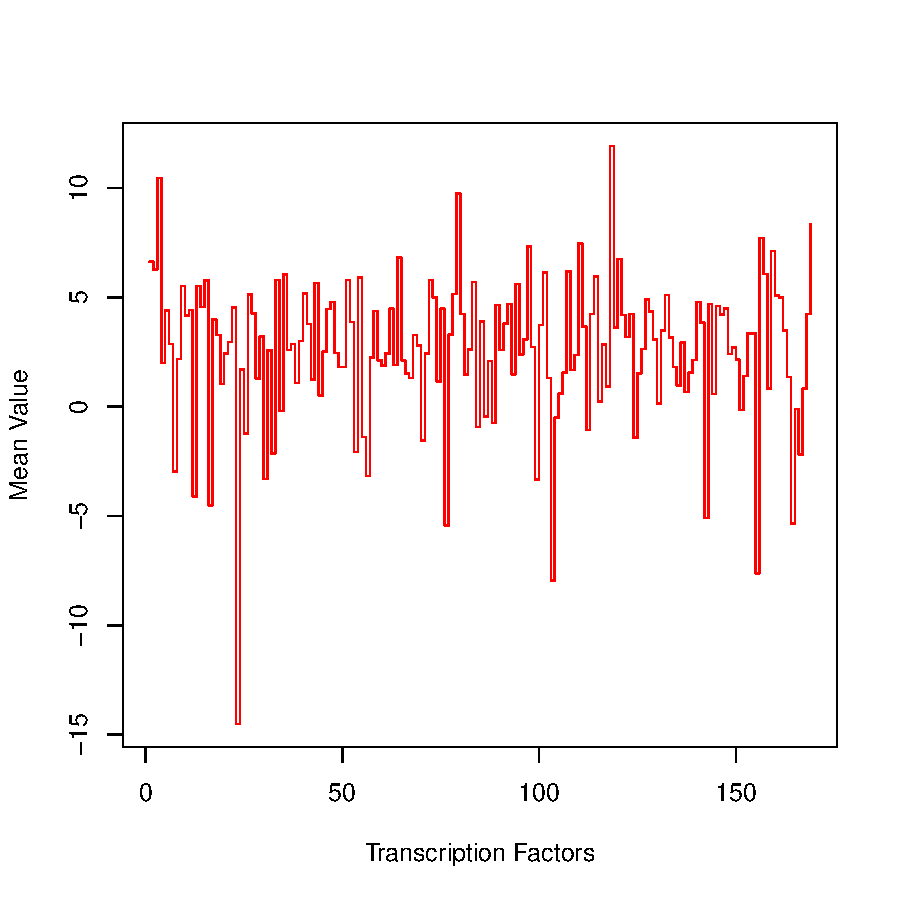
\includegraphics{chipDyno-figure1}
\caption{Mean}
\label{valMin}
\end{figure}

%\begin{figure}
%<<figure2, fig=TRUE, height=3, width= 3>>=
%#image(Sigma[1:40,1:40])
%heatmap(Sigma[1:30,1:30], Rowv=NA, Colv=NA, col = heat.colors(256),  margins=c(2,2))
%@
%\caption{Sigma[1:40,1:40]}
%\label{valSigma}
%\end{figure}

%---------------------------------------------------------
\section{Computation of posterior expectations for a given gene and TF}
%---------------------------------------------------------
\Rfunction{chipDynoStatPostEst} and \Rfunction{chipDynoStatPostEstNoise} computes posterior expectations of transcription factor activity for a transcription factor and a gene given the uncertainty of the expression level is absent or present respectively.


\begin{Schunk}
\begin{Sinput}
> #rm(list=ls())
> load("/home/muhammad/Dropbox/Git/mlprojects/chipDyno/R/ResultsTu_New_10000Ita_Lovelace.RData")
> source("/home/muhammad/Dropbox/Git/mlprojects/chipDyno/R/chipDynoLoadModules.R")
> annotations = annotation
> transNames=TransNames
> transName= "ACE2"
> geneName="YHR143W"
> #geneName="KRE32"
> 
> npts=ncol(data);
> nTrans=ncol(X);
> c = class(geneName)
> v= mat.or.vec(length(annotations),1)
> if (c == 'character'){
+   for (i in 1: nrow(annotations)) { 
+ 		v[i] <- geneName==annotations[i,1]
+ 		}
+ 	x=data.matrix(X[which(v==1),])
+ 	data=t(data[which(v==1),])
+ 	precs = precs[which(v==1),]
+ 
+ } else if (c=='integer'){
+ 	x=data.matrix(X[geneName,])
+ 	data=data[geneName,]
+ 	precs=precs[geneName,] ### t() ???
+ 
+ } else {
+ 	print('Error: Genes can be identified either by number or name')
+ }
> expectations=chipDynoStatPostEstNoise(data,x,Sigma,beta,precs,gamma,mu);
> expectations.b=expectations[[1]];
> expectations.tfError=expectations[[2]];
> expectations.tfErrorDiffs=expectations[[3]];
> index=which(transName==transNames);
> if (x[index,]== 0) {
+  print('Error: The gene selected is not a target of the transcription factor')
+ }
> tf=expectations.b[,index];
> ind=which(transName == transNames[which(x!=0)]);
> tfErrors=expectations.tfError[,ind];
> tfErrorsDiffs=expectations.tfErrorDiffs[,,ind];
> tf
\end{Sinput}
\begin{Soutput}
 [1] 0.6842732 1.2928971 2.4140684 2.5589165 2.5752429 2.5505454 2.1369019 1.6541770
 [9] 2.0730713 1.0057944 0.9698620 0.9217374 0.7920417 1.5490587 2.6194954 2.5186103
[17] 2.3162395 2.6597092 2.2073021 1.7778347 1.2716619 1.2455317 1.4295381 1.0507008
[25] 0.9321431 1.9023200 2.4522094 2.7434556 2.4750629 2.3039070 2.1068440 2.1683739
[33] 1.6146242 1.3278398 1.2193253 0.8508893
\end{Soutput}
\begin{Sinput}
> tfErrors
\end{Sinput}
\begin{Soutput}
 [1] 3.727733 3.717664 3.715976 3.715939 3.715935 3.715940 3.716087 3.716601 3.716115
[10] 3.720425 3.719345 3.719530 3.726181 3.716770 3.715925 3.715949 3.716008 3.715919
[19] 3.716061 3.716406 3.717766 3.717919 3.717099 3.719184 3.723853 3.716255 3.715964
[28] 3.715908 3.715957 3.716015 3.716106 3.716059 3.716676 3.717461 3.717833 3.721902
\end{Soutput}
\end{Schunk}

%\begin{figure}
%<<figure3, fig=TRUE>>=
%par(mfcol=c(1,3))
%image(Z, col=pal.1(100))
%image(expectations.tfErrorDiffs[,,ind], col = heat.colors(50))
%heatmap(expectations.tfErrorDiffs[,,2])
%@
%\caption{Covariance Matrix}
%\label{Cov_image}
%\end{figure}

%---------------------------------------------------------
\section{Posterior expectations for a given TF : chipDynoExpectationsFastNoise}
%---------------------------------------------------------
\Rfunction{chipDynoExpectationsFast} and \Rfunction{chipDynoExpectationsFastNoise} computes posterior expectations of transcription factor activity for a given transcription factor considering uncertainty of the expression level  absent or present respectively. These functions first find all the genes gegulated by geven transcription factor and later the activity on different genes. The format of the function and arguments are-



\begin{figure}
\begin{Schunk}
\begin{Sinput}
> M <- matrix(c(rep(1:4)), byrow=TRUE, nrow=2) # Choose the position by matrix setting!
> layout(M) 
> k <- c(46,47,50,52)
> #for (i in 1:4){
> for (i in k){
+ #expectations = chipDynoExpectationsFast(data,X,Sigma,beta,gamma,mu, 
+ #                    transNames, annotations, name, genesIn[i]);
+ expectations = chipDynoExpectationsFastNoise(data,X,Sigma,beta,precs, 
+                     gamma,mu, transNames, annotations, name, genesIn[i]);
+ TF[i,] = expectations[[1]];
+ TFError[i,] = expectations[[2]];
+ gnName=annotation[genesIn[i]]
+ plotErrorBar(TF[i,],TFError[i,], gnName)
+ }
\end{Sinput}
\end{Schunk}
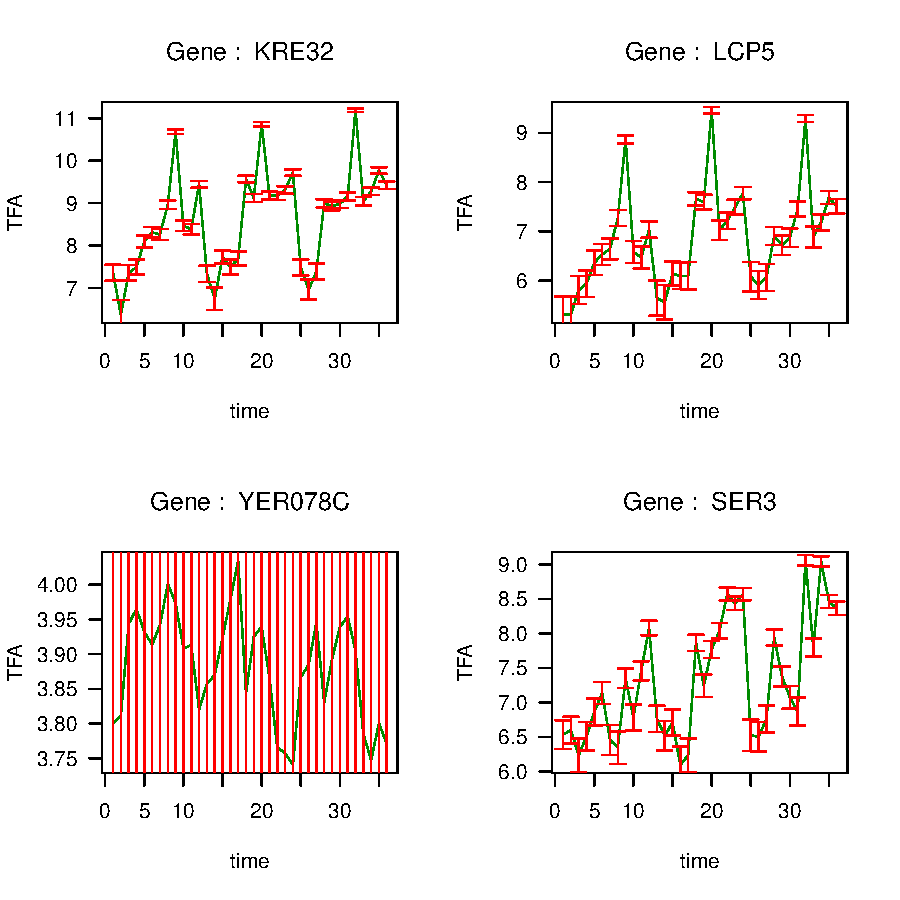
\includegraphics{chipDyno-figure4}
\caption{TFA Activities}
\label{TFA_activiitys}
\end{figure}
%...................................

\begin{Schunk}
\begin{Sinput}
> rm(list=ls())
> load("ResultsSpellman_200Ita.RData")
> #load("/home/muhammad/Dropbox/Git/mlprojects/chipDyno/R/ResultsTu_New_10000Ita_Lovelace.RData")
> source("/home/muhammad/Dropbox/Git/mlprojects/chipDyno/R/chipDynoLoadModules.R")
> transNames = TransNames
> annotations = annotation
> nTrans=nrow(TransNames);
> lst=list();
> newX=array(0, dim <-c(dim(X)));
> newXVals=array(0, dim <-c(dim(X)));
> #i=2; name=TransNames[i,] # ACE2 for demSpellman
> 
> name="ACE2"
> index=which(name == transNames);
> genesIn=which(X[,index]!=0);
> anno=annotations[which(X[,index]!=0)];
> nTargets=length(anno);
> npts=ncol(data);
> TF=array(0, dim=c(nTargets,npts));
> TFError=array(0, dim=c(nTargets,npts));
> TFErrorDiff=array(0, dim=c(npts,npts,nTargets));
> plotErrorBar <- function(y,SE, gnName){
+  
+ add.error.bars <- function(x,y,SE,w,col=1){
+  x0 = x; y0 = (y-SE); x1 =x; y1 = (y+SE);
+  arrows(x0, y0, x1, y1, code=3,angle= 90,length=w,col=col);
+  }
+  
+ x <- c(1:length(y));
+ plot(x,y, type = 'l', col='green4', las=1, xlab="time", ylab="TFA", 
+       main=bquote("Gene : " ~ .(gnName)));
+ add.error.bars(x,y,SE,0.05,col='red');
+ }
\end{Sinput}
\end{Schunk}

\begin{figure}
\begin{Schunk}
\begin{Sinput}
> M <- matrix(c(rep(1:4)), byrow=TRUE, nrow=2) # Choose the position by matrix setting!
> layout(M) 
> k <- c(17,19, 28, 50)
> #for (i in 8:11){
> for (i in k){
+ expectations = chipDynoExpectationsFast(data,X,Sigma,beta,gamma,mu, transNames, annotations, name, genesIn[i]);
+ #expectations = chipDynoExpectationsFastNoise(data,X,Sigma,beta,precs, gamma,mu, transNames, annotations, name, genesIn[i]);
+ TF[i,] = expectations[[1]];
+ TFError[i,] = expectations[[2]];
+ gnName=annotation[genesIn[i]]
+ 
+ plotErrorBar(TF[i,],TFError[i,], gnName)
+ }
\end{Sinput}
\end{Schunk}
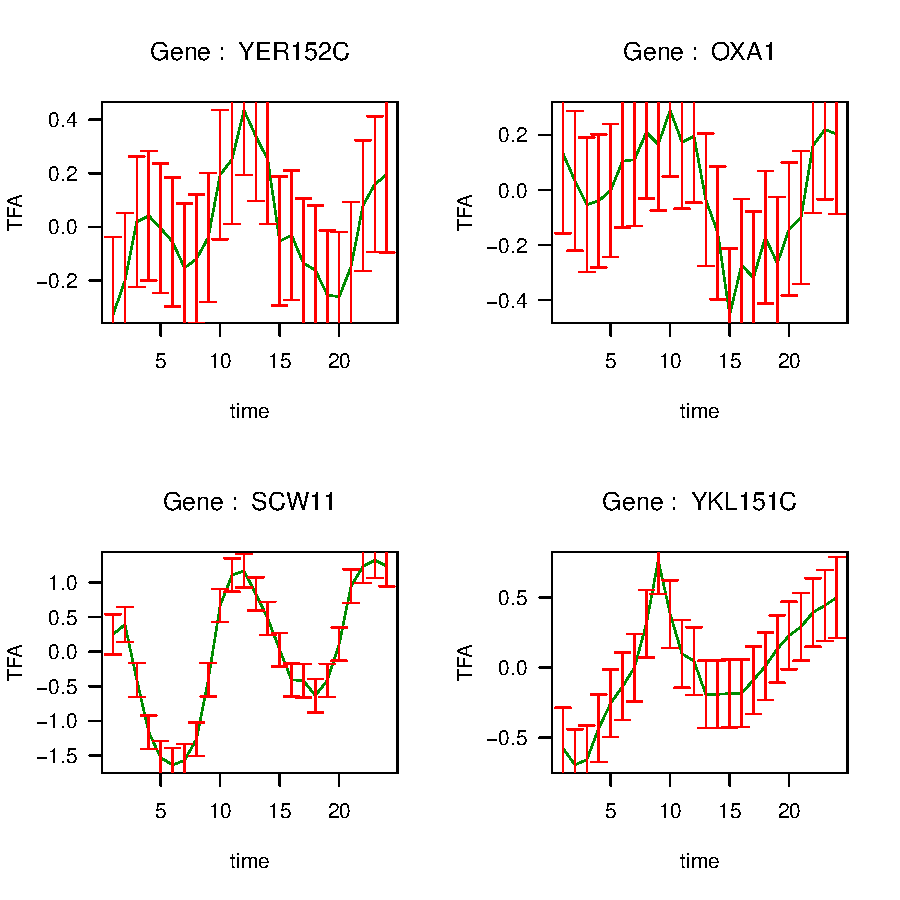
\includegraphics{chipDyno-figure5}
\caption{TFA Activities of ACE2}
\label{TFA_activities_ACE2}
\end{figure}

%---------------------------------------------------------
\section{Maximum Transcription Factor Activity}
%---------------------------------------------------------
\Rfunction{chipDynoMaxDiff} computes the maximum transcription factor activity of all the target or transcribed genes for a given transcription factor. For a specific target it also computes the variation over time.


\begin{Schunk}
\begin{Sinput}
> rm(list=ls())
> load("/home/muhammad/Dropbox/Git/mlprojects/chipDyno/R/ResultsTu_New_10000Ita_Lovelace.RData")
> source("/home/muhammad/Dropbox/Git/mlprojects/chipDyno/R/chipDynoLoadModules.R")
> transNames = TransNames
> annotations = annotation
> nTrans=nrow(TransNames);
> lst=list();
> newX=array(0, dim <-c(dim(X)));
> newXVals=array(0, dim <-c(dim(X)));
> i=6; # TransNames[6,] is "AFT2"
> expectations =chipDynoTransFactNoise(data,X,Sigma,beta,precs, gamma, mu, 
+   					TransNames, annotation, TransNames[i,]);
> TF = expectations[[1]]
> TFError = expectations [[2]]
> TFErrorDiff = expectations [[3]]
> maxVars=chipDynoMaxDiff(TF,TFErrorDiff);
> #maxVars
\end{Sinput}
\end{Schunk}


\begin{figure}
\begin{Schunk}
\begin{Sinput}
> par(mfrow=c(2,2))
> image(diffs[,,1],col = heat.colors(50), main = "Target 1: Variation over time ")
> image(diffs[,,4],col = heat.colors(50), main = "Target 4: Variation over time ")
> image(TFErrorDiff[,,4], col = heat.colors(50), main = "TF Error difference for Target 4")
> image((diffs[,,4]/TFErrorDiff[,,4]), col = heat.colors(50), main = "diffs/TFErrorDiff")
\end{Sinput}
\end{Schunk}
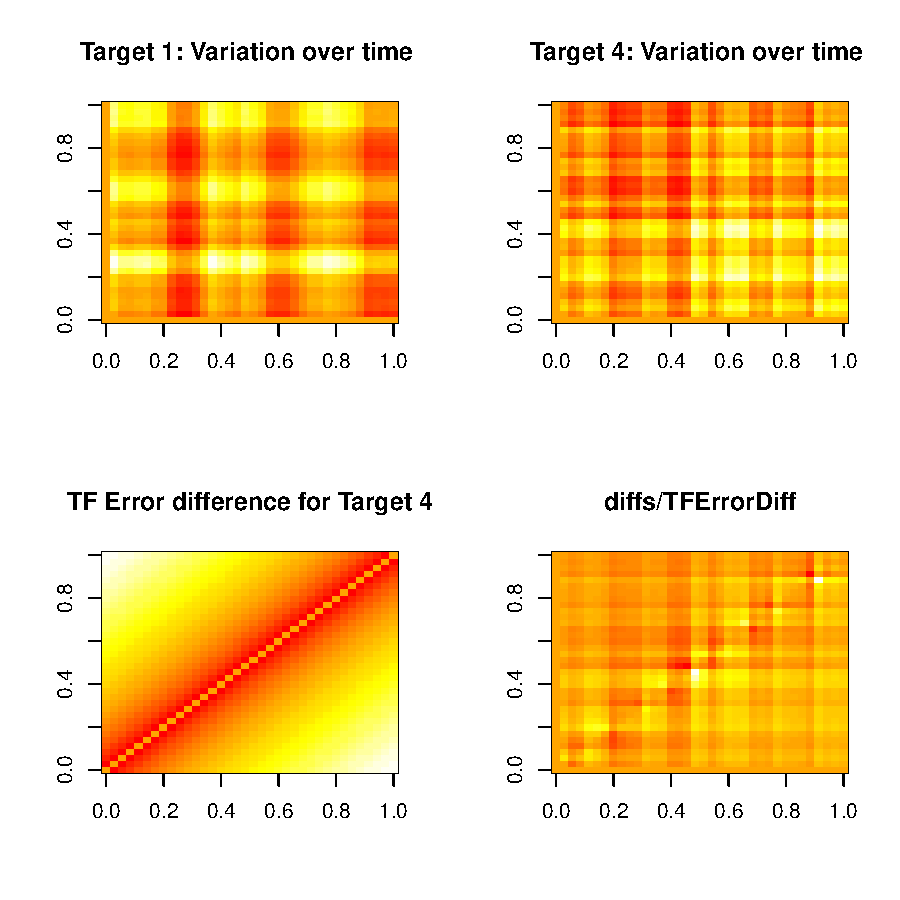
\includegraphics{chipDyno-figure6}
\caption{Error Difference}
\label{Error_Diff}
\end{figure}


%---------------------------------------------------------
\section{TFAs with error bars :chipDynoTransFactNoise}
%---------------------------------------------------------
\Rfunction{chipDynoTransFactNoise} provides transcription factor activities with error margin for a given transcription factor. For an example we are interested to find the activity of transcription factor \Rcode{ACE2}. Using \Rfunction{chipDynoTransFactNoise} we can find it by following way-


\begin{Schunk}
\begin{Sinput}
> rm(list=ls())
> load("/home/muhammad/Dropbox/Git/mlprojects/chipDyno/R/ResultsTu_New_10000Ita_Lovelace.RData")
> #load("/home/muhammad/Dropbox/Git/mlprojects/chipDyno/R/ResultsTu.RData")
> source("/home/muhammad/Dropbox/Git/mlprojects/chipDyno/R/chipDynoLoadModules.R")
> i=4; TransNames[i,]
\end{Sinput}
\begin{Soutput}
[1] "ACE2"
\end{Soutput}
\begin{Sinput}
> expectations =chipDynoTransFactNoise(data,X,Sigma,beta, precs, gamma, mu,
+                                      TransNames, annotation, TransNames[i,]);
> TransNames[i,] # Name of the transcription factor
\end{Sinput}
\begin{Soutput}
[1] "ACE2"
\end{Soutput}
\begin{Sinput}
> expectations[[1]][1:5,1:5] # Transcription facot activity on different genes
\end{Sinput}
\begin{Soutput}
           [,1]       [,2]       [,3]       [,4]       [,5]
[1,]  1.0091035  1.4175891  1.9475555  2.1090371  2.1435868
[2,]  3.0003668  2.8129669  2.6342091  2.8765482  2.9749977
[3,] -0.8578099 -0.5649832 -0.7160508 -0.7109128 -0.6853118
[4,]  0.3080097  0.3915622  0.2879910  0.2844155  0.2870976
[5,]  2.1289532  2.1274012  2.1685124  2.1869350  2.1438690
\end{Soutput}
\begin{Sinput}
> expectations[[2]][1:5,1:5] # Transcription facot activity error on different genes
\end{Sinput}
\begin{Soutput}
         [,1]     [,2]     [,3]     [,4]     [,5]
[1,] 3.670207 3.669784 3.669675 3.669663 3.669661
[2,] 3.525075 3.525175 3.525346 3.525134 3.525078
[3,] 4.601053 4.600577 4.600710 4.600684 4.600709
[4,] 4.600519 4.600514 4.600520 4.600520 4.600520
[5,] 4.968442 4.968441 4.968450 4.968453 4.968447
\end{Soutput}
\begin{Sinput}
> #expectations[[2]]
\end{Sinput}
\end{Schunk}


%---------------------------------------------------------
\section{Significantly varying TFs :chipDynoActTransFactNoise}
%---------------------------------------------------------
\Rfunction{chipDynoActTransFact} and \Rfunction{chipDynoActTransFactNoise} can find out transcription factor activity for all the transcription factors without or with uncertainty of expression level respectively 



\begin{Schunk}
\begin{Sinput}
> rm(list=ls())
> load("/home/muhammad/Dropbox/Git/mlprojects/chipDyno/R/ResultsTu_New_10000Ita_Lovelace.RData")
> source("/home/muhammad/Dropbox/Git/mlprojects/chipDyno/R/chipDynoLoadModules.R")
> nTrans=nrow(TransNames);
> lst=list();
> newX=array(0, dim <-c(dim(X)));
> newXVals=array(0, dim <-c(dim(X)));
> i=1
> expectations =chipDynoTransFactNoise(data,X,Sigma,beta,precs, gamma, mu, 
+   					TransNames, annotation, TransNames[i,]);
> expectations[[1]][1:5,1:5] # Transcription Factor activity
\end{Sinput}
\begin{Soutput}
         [,1]     [,2]      [,3]      [,4]     [,5]
[1,] 1.181507 1.194267 0.9405349 0.8873723 1.002965
[2,] 7.993588 9.051546 8.8765448 8.8233255 9.227746
[3,] 6.273973 6.260386 5.8544201 5.9010941 6.423778
[4,] 9.366391 8.709048 7.5041669 7.3267449 7.651604
[5,] 4.130014 4.159660 3.7399778 4.1997017 4.597343
\end{Soutput}
\begin{Sinput}
> expectations[[2]][1:5,1:5] # Transcription Factor activity error
\end{Sinput}
\begin{Soutput}
           [,1]      [,2]      [,3]      [,4]      [,5]
[1,] 4.11673886 4.1165627 4.1182251 4.1181800 4.1188190
[2,] 0.19176468 0.1223281 0.1336542 0.1345851 0.1191347
[3,] 0.23710986 0.2259855 0.2924871 0.2783009 0.2350629
[4,] 0.09052251 0.1131770 0.1928447 0.2006229 0.1855977
[5,] 4.05516555 4.0551077 4.0559909 4.0550716 4.0547750
\end{Soutput}
\begin{Sinput}
> expectations[[3]][1:5,1:5,1] # Transcription Factor activity error difference
\end{Sinput}
\begin{Soutput}
          [,1]      [,2]      [,3]      [,4]      [,5]
[1,] 1.0000000 0.4468329 0.6234075 0.7537601 0.8651675
[2,] 0.4468329 1.0000000 0.4532274 0.6226605 0.7550226
[3,] 0.6234075 0.4532274 1.0000000 0.4597133 0.6301797
[4,] 0.7537601 0.6226605 0.4597133 1.0000000 0.4620770
[5,] 0.8651675 0.7550226 0.6301797 0.4620770 1.0000000
\end{Soutput}
\end{Schunk}


%---------------------------------------------------------
\section{Given Gene: lists activators in decreasing order}
%---------------------------------------------------------
For a given gene we can find out the list of activators using the function \Rfunction{chipDynoGeneActNoise}. It will list all the activators in decreasing order with transcription factor activity and activity error.


\begin{Schunk}
\begin{Sinput}
> rm(list=ls())
> load("/home/muhammad/Dropbox/Git/mlprojects/chipDyno/R/ResultsTu_New_10000Ita_Lovelace.RData")
> source("/home/muhammad/Dropbox/Git/mlprojects/chipDyno/R/chipDynoLoadModules.R")
> geneName="YHR143W"; 
> #geneName="AGA1"; 
> transNames=TransNames
> activators = chipDynoGeneActNoise(data, X, Sigma, beta, precs, gamma,mu, 
+                     transNames, annotation, geneName)
> activators[[1]] # List of activators
\end{Sinput}
\begin{Soutput}
[1] "ACE2" "FKH2" "FKH1" "MBP1"
\end{Soutput}
\begin{Sinput}
> activators[[2]] # Maximum transcription factor activity
\end{Sinput}
\begin{Soutput}
[1] 0.78852602 0.78235753 0.55227342 0.06221002
\end{Soutput}
\begin{Sinput}
> activators[[3]] # Maximum transcription factor activity error
\end{Sinput}
\begin{Soutput}
[1] 3.715908 3.925077 4.405851 5.262743
\end{Soutput}
\end{Schunk}


%---------------------------------------------------------
%\section{Sectioning: this is a section}
%---------------------------------------------------------

%\subsection{This is a subsection}
%!!!!!!!!!!

%\subsubsection{This is a subsubsection}
%?@?@?@? 
%---------------------------------------------------------
%\section{Including a figure}
%---------------------------------------------------------


%---------------------------------------------------------
\section{Session info}
%---------------------------------------------------------
Here is the output of \Rfunction{sessionInfo} on the system on which
this document was compiled:
\begin{Schunk}
\begin{Sinput}
> toLatex(sessionInfo())
\end{Sinput}
\begin{itemize}\raggedright
  \item R version 3.0.2 (2013-09-25), \verb|x86_64-pc-linux-gnu|
  \item Locale: \verb|LC_CTYPE=en_GB.UTF-8|, \verb|LC_NUMERIC=C|, \verb|LC_TIME=en_GB.UTF-8|, \verb|LC_COLLATE=en_GB.UTF-8|, \verb|LC_MONETARY=en_GB.UTF-8|, \verb|LC_MESSAGES=en_GB.UTF-8|, \verb|LC_PAPER=en_GB.UTF-8|, \verb|LC_NAME=C|, \verb|LC_ADDRESS=C|, \verb|LC_TELEPHONE=C|, \verb|LC_MEASUREMENT=en_GB.UTF-8|, \verb|LC_IDENTIFICATION=C|
  \item Base packages: base, datasets, graphics, grDevices, methods, stats,
    utils
  \item Other packages: Matrix~1.1-1.1
  \item Loaded via a namespace (and not attached): BiocStyle~0.0.19, grid~3.0.2,
    lattice~0.20-24, tools~3.0.2
\end{itemize}\end{Schunk}


%\bibliographystyle{abbrv}
%\bibliographystyle{alpha}
\bibliographystyle{apalike}

\bibliography{bib_chipDyno}

\end{document}
